\documentclass[journal,12pt,twocolumn]{IEEEtran}
%
\usepackage{setspace}
\usepackage{gensymb}
\usepackage{xcolor}
\usepackage{caption}
%\usepackage{subcaption}
%\doublespacing
\singlespacing

%\usepackage{graphicx}
%\usepackage{amssymb}
%\usepackage{relsize}
\usepackage[cmex10]{amsmath}
\usepackage{mathtools}
%\usepackage{amsthm}
%\interdisplaylinepenalty=2500
%\savesymbol{iint}
%\usepackage{txfonts}
%\restoresymbol{TXF}{iint}
%\usepackage{wasysym}
\usepackage{hyperref}
\usepackage{amsthm}
\usepackage{mathrsfs}
\usepackage{txfonts}
\usepackage{stfloats}
\usepackage{cite}
\usepackage{cases}
\usepackage{subfig}
%\usepackage{xtab}
\usepackage{longtable}
\usepackage{multirow}
%\usepackage{algorithm}
%\usepackage{algpseudocode}
%\usepackage{enumerate}-get 
\usepackage{enumitem}
\usepackage{mathtools}
%\usepackage{iithtlc}
%\usepackage[framemethod=tikz]{mdframed}
\usepackage{listings}
\usepackage{polynom}


%\usepackage{stmaryrd}


%\usepackage{wasysym}
%\newcounter{MYtempeqncnt}
\DeclareMathOperator*{\Res}{Res}
%\renewcommand{\baselinestretch}{2}
\renewcommand\thesection{\arabic{section}}
\renewcommand\thesubsection{\thesection.\arabic{subsection}}
\renewcommand\thesubsubsection{\thesubsection.\arabic{subsubsection}}

\renewcommand\thesectiondis{\arabic{section}}
\renewcommand\thesubsectiondis{\thesectiondis.\arabic{subsection}}
\renewcommand\thesubsubsectiondis{\thesubsectiondis.\arabic{subsubsection}}

%\renewcommand{\labelenumi}{\textbf{\theenumi}}
%\renewcommand{\theenumi}{P.\arabic{enumi}}

% correct bad hyphenation here
\hyphenation{op-tical net-works semi-conduc-tor}

\lstset{
language=Python,
frame=single, 
breaklines=true,
columns=fullflexible
}



\begin{document}
%

\theoremstyle{definition}
\newtheorem{theorem}{Theorem}[section]
\newtheorem{problem}{Problem}
\newtheorem{proposition}{Proposition}[section]
\newtheorem{lemma}{Lemma}[section]
\newtheorem{corollary}[theorem]{Corollary}
\newtheorem{example}{Example}[section]
\newtheorem{definition}{Definition}[section]
%\newtheorem{algorithm}{Algorithm}[section]
%\newtheorem{cor}{Corollary}
\newcommand{\BEQA}{\begin{eqnarray}}
\newcommand{\EEQA}{\end{eqnarray}}
\newcommand{\define}{\stackrel{\triangle}{=}}
\bibliographystyle{IEEEtran}
%\bibliographystyle{ieeetr}
\providecommand{\nCr}[2]{\,^{#1}C_{#2}} % nCr
\providecommand{\nPr}[2]{\,^{#1}P_{#2}} % nPr
\providecommand{\mbf}{\mathbf}
\providecommand{\pr}[1]{\ensuremath{\Pr\left(#1\right)}}
\providecommand{\qfunc}[1]{\ensuremath{Q\left(#1\right)}}
\providecommand{\sbrak}[1]{\ensuremath{{}\left[#1\right]}}
\providecommand{\lsbrak}[1]{\ensuremath{{}\left[#1\right.}}
\providecommand{\rsbrak}[1]{\ensuremath{{}\left.#1\right]}}
\providecommand{\brak}[1]{\ensuremath{\left(#1\right)}}
\providecommand{\lbrak}[1]{\ensuremath{\left(#1\right.}}
\providecommand{\rbrak}[1]{\ensuremath{\left.#1\right)}}
\providecommand{\cbrak}[1]{\ensuremath{\left\{#1\right\}}}
\providecommand{\lcbrak}[1]{\ensuremath{\left\{#1\right.}}
\providecommand{\rcbrak}[1]{\ensuremath{\left.#1\right\}}}
\theoremstyle{remark}
\newtheorem{rem}{Remark}
\newcommand{\sgn}{\mathop{\mathrm{sgn}}}
\providecommand{\abs}[1]{\left\vert#1\right\vert}
\providecommand{\res}[1]{\Res\displaylimits_{#1}} 
\providecommand{\norm}[1]{\lVert#1\rVert}
\providecommand{\mtx}[1]{\mathbf{#1}}
\providecommand{\mean}[1]{E\left[ #1 \right]}
\providecommand{\fourier}{\overset{\mathcal{F}}{ \rightleftharpoons}}
\providecommand{\ztrans}{\overset{\mathcal{Z}}{ \rightleftharpoons}}
%\providecommand{\hilbert}{\overset{\mathcal{H}}{ \rightleftharpoons}}
\providecommand{\system}{\overset{\mathcal{H}}{ \longleftrightarrow}}
	%\newcommand{\solution}[2]{\textbf{Solution:}{#1}}
\newcommand{\solution}{\noindent \textbf{Solution: }}
\providecommand{\dec}[2]{\ensuremath{\overset{#1}{\underset{#2}{\gtrless}}}}
\numberwithin{equation}{section}
%\numberwithin{equation}{subsection}
%\numberwithin{problem}{subsection}
%\numberwithin{definition}{subsection}
\newcommand{\myvec}[1]{\ensuremath{\begin{pmatrix}#1\end{pmatrix}}}
\newcommand{\mymat}[1]{\ensuremath{\begin{bmatrix}#1\end{bmatrix}}}
\newcommand{\mydet}[1]{\ensuremath{\begin{vmatrix}#1\end{vmatrix}}}

\makeatletter
\def\pld@CF@loop#1+{%
    \ifx\relax#1\else
        \begingroup
          \pld@AccuSetX11%
          \def\pld@frac{{}{}}\let\pld@symbols\@empty\let\pld@vars\@empty
          \pld@false
          #1%
          \let\pld@temp\@empty
          \pld@AccuIfOne{}{\pld@AccuGet\pld@temp
                            \edef\pld@temp{\noexpand\pld@R\pld@temp}}%
           \pld@if \pld@Extend\pld@temp{\expandafter\pld@F\pld@frac}\fi
           \expandafter\pld@CF@loop@\pld@symbols\relax\@empty
           \expandafter\pld@CF@loop@\pld@vars\relax\@empty
           \ifx\@empty\pld@temp
               \def\pld@temp{\pld@R11}%
           \fi
          \global\let\@gtempa\pld@temp
        \endgroup
        \ifx\@empty\@gtempa\else
            \pld@ExtendPoly\pld@tempoly\@gtempa
        \fi
        \expandafter\pld@CF@loop
    \fi}
\def\pld@CMAddToTempoly{%
    \pld@AccuGet\pld@temp\edef\pld@temp{\noexpand\pld@R\pld@temp}%
    \pld@CondenseMonomials\pld@false\pld@symbols
    \ifx\pld@symbols\@empty \else
        \pld@ExtendPoly\pld@temp\pld@symbols
    \fi
    \ifx\pld@temp\@empty \else
        \pld@if
            \expandafter\pld@IfSum\expandafter{\pld@temp}%
               {\expandafter\def\expandafter\pld@temp\expandafter
                    {\expandafter\pld@F\expandafter{\pld@temp}{}}}%
                {}%
        \fi
        \pld@ExtendPoly\pld@tempoly\pld@temp
        \pld@Extend\pld@tempoly{\pld@monom}%
    \fi}            
\@addtoreset{figure}{problem}
\makeatother
\lstset{
language=Python,
frame=single, 
breaklines=true,
columns=fullflexible
}
\let\StandardTheFigure\thefigure
%\renewcommand{\thefigure}{\theproblem.\arabic{figure}}
\renewcommand{\thefigure}{\theproblem}
%\numberwithin{figure}{subsection}
\def\putbox#1#2#3{\makebox[0in][l]{\makebox[#1][l]{}\raisebox{\baselineskip}[0in][0in]{\raisebox{#2}[0in][0in]{#3}}}}
     \def\rightbox#1{\makebox[0in][r]{#1}}
     \def\centbox#1{\makebox[0in]{#1}}
     \def\topbox#1{\raisebox{-\baselineskip}[0in][0in]{#1}}
     \def\midbox#1{\raisebox{-0.5\baselineskip}[0in][0in]{#1}}
\vspace{3cm}
\title{ 
%\logo{
Digital Signal Processing
%}
%	\logo{Octave for Math Computing }
}
\author{AI21BTECH11016 \\ Blessy Anvitha J} 

\maketitle
%\newpage
\tableofcontents
%\renewcommand{\thefigure}{\thesection.\theenumi}
%\renewcommand{\thetable}{\thesection.\theenumi}
\renewcommand{\thefigure}{\theenumi}
\renewcommand{\thetable}{\theenumi}
\renewcommand{\vec}{\textbf}
%\renewcommand{\theequation}{\thesection}
\bigskip
\section{Software Installation}
Run the following commands
\begin{lstlisting}
sudo apt-get update
sudo apt-get install libffi-dev libsndfile1 python3-scipy  python3-numpy python3-matplotlib 
sudo pip install cffi pysoundfile 
\end{lstlisting}
\section{Digital Filter}
\begin{enumerate}[label=\thesection.\arabic*
,ref=\thesection.\theenumi]
\item
\label{prob:input}
Download the sound file from  
\begin{lstlisting}
https://github.com/JBA-12/EE3900/blob/main/A1/codes/Sound_Noise.wav
\end{lstlisting}
%\href{http://tlc.iith.ac.in/img/sound/Sound_Noise.wav}{\url{http://tlc.iith.ac.in/img/sound/Sound_Noise.wav}}  
%in the link given below.
%\linebreak
\item
\label{prob:spectrogram}
You will find a spectrogram at \href{https://academo.org/demos/spectrum-analyzer}{\url{https://academo.org/demos/spectrum-analyzer}}. 
%\end{problem}
%%
%
%%\onecolumn
%%\input{./figs/fir}
%\begin{problem}
Upload the sound file that you downloaded in Problem \ref{prob:input} in the spectrogram  and play.  Observe the spectrogram. What do you find?
\\
%
\solution There are a lot of yellow lines between 440 Hz to 5.1 KHz.  These represent the synthesizer key tones. Also, the key strokes
are audible along with background noise.
% By observing spectrogram, it clearly shows that tonal frequency is under 4kHz. And above 4kHz only noise is present.
\item
\label{prob:output}
Write the python code for removal of out of band noise and execute the code.
\\
\solution The following code removes the out of band noise
\begin{lstlisting}
https://github.com/JBA-12/EE3900/blob/main/A1/codes/2.3.py
\end{lstlisting}
and execute the code using the following command
\begin{lstlisting}
python3 2.3.py
\end{lstlisting}
%\begin{figure}[h]
%\centering
%\includegraphics[width=\columnwidth]{enc_block_diag.png}
%\caption{}
%\label{fig:convolution encoder}
%\end{figure}
%\input{block_enc}
\item
The output of the python script in Problem \ref{prob:output} is the audio file Sound\_With\_ReducedNoise.wav. Play the file in the spectrogram in Problem \ref{prob:spectrogram}. What do you observe?
\\
\solution The key strokes as well as background noise is subdued in the audio.  Also,  the signal is blank for frequencies above 5.1 kHz.
\end{enumerate}
\section{Difference Equation}
\begin{enumerate}[label=\thesection.\arabic*,ref=\thesection.\theenumi]
\item Let
\label{def:xn}
\begin{equation}
x(n) = \cbrak{\underset{\uparrow}{1},2,3,4,2,1}
\end{equation}
Sketch $x(n)$.
\item Let
\begin{multline}
\label{eq:iir_filter}
y(n) + \frac{1}{2}y(n-1) = x(n) + x(n-2), 
\\
 y(n) = 0, n < 0
\end{multline}
Sketch $y(n)$.
\\
\solution The following code yields Fig. \ref{fig:xnyn}.
\begin{lstlisting}
https://github.com/JBA-12/EE3900/blob/main/A1/codes/3.2.py
\end{lstlisting}
and run the code using the following command
\begin{lstlisting}
python3 3.2.py
\end{lstlisting}
\begin{figure}[!ht]
\begin{center}
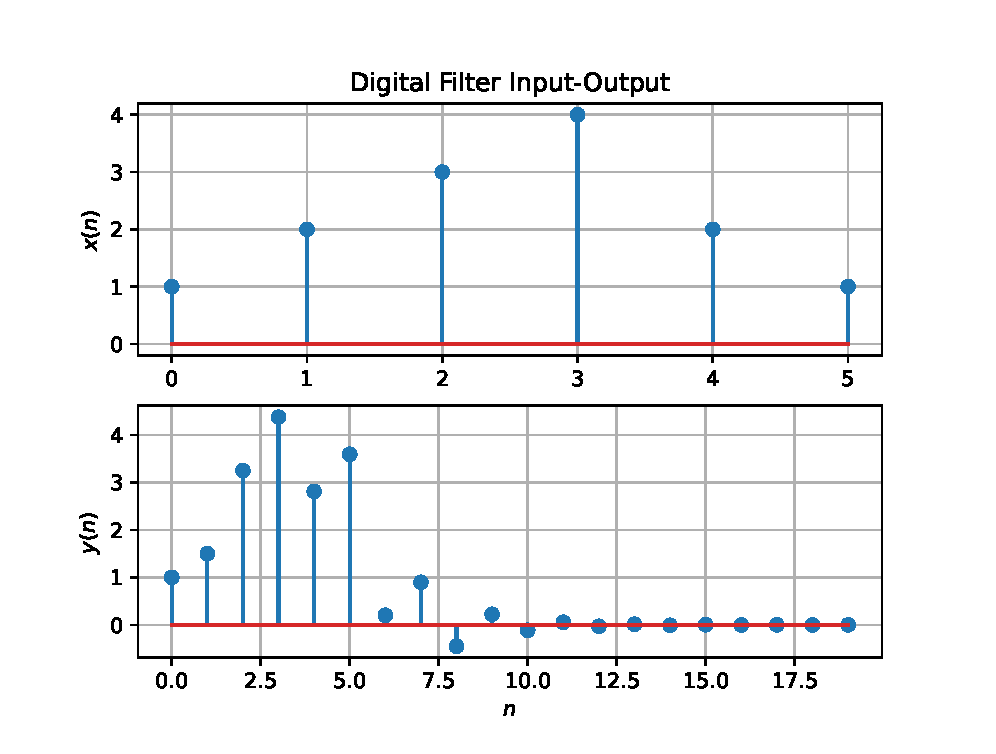
\includegraphics[width=\columnwidth]{./figs/xnyn}
\end{center}
\captionof{figure}{}
\label{fig:xnyn}	
\end{figure}
\item Repeat the above exercise using a C code.
\solution The following C code yields y(n).dat file
\begin{lstlisting}
https://github.com/JBA-12/EE3900/blob/main/A1/codes/3.3.c
\end{lstlisting}
and run the code using the following commands
\begin{lstlisting}
gcc 3.3.c 
./a.out
\end{lstlisting}
The following python code inputs y(n) produced using C code and yields Fig. \ref{fig:3.3}.
\begin{lstlisting}
https://github.com/JBA-12/EE3900/blob/main/A1/codes/3.3.py
\end{lstlisting}
and run the code using the following command
\begin{lstlisting}
python3 3.3.py
\end{lstlisting}
\begin{figure}[!ht]
\begin{center}
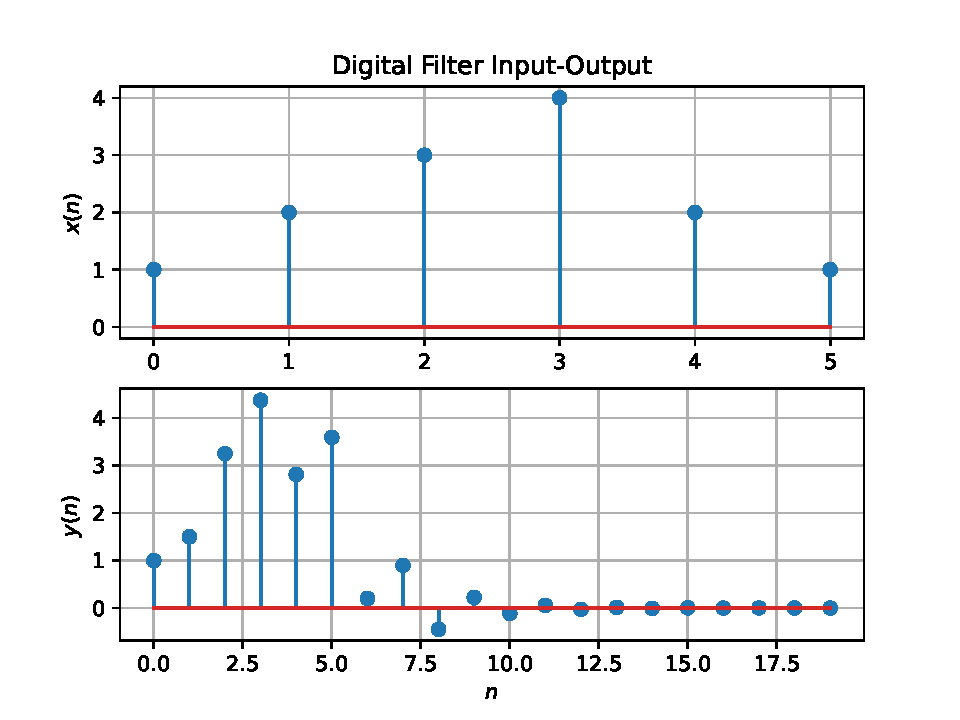
\includegraphics[width=\columnwidth]{./figs/3.3}
\end{center}
\captionof{figure}{}
\label{fig:3.3}	
\end{figure}
\end{enumerate}
\section{$Z$-transform}
\begin{enumerate}[label=\thesection.\arabic*]
\item The $Z$-transform of $x(n)$ is defined as
%
\begin{equation}
\label{eq:z_trans}
X(z)={\mathcal {Z}}\{x(n)\}=\sum _{n=-\infty }^{\infty }x(n)z^{-n}
\end{equation}
%
Show that
\begin{equation}
\label{eq:shift1}
{\mathcal {Z}}\{x(n-1)\} = z^{-1}X(z)
\end{equation}
and find
\begin{equation}
	{\mathcal {Z}}\{x(n-k)\} 
\end{equation}
\solution From \eqref{eq:z_trans},
\begin{align}
{\mathcal {Z}}\{x(n-k)\} &=\sum _{n=-\infty }^{\infty }x(n-k)z^{-n}
\end{align}
substitute n - k = t
\begin{align}
{\mathcal {Z}}\{x(n-k)\} &=\sum _{n=-\infty }^{\infty }x(n)z^{-n-k}\\ &= z^{-k}\sum _{n=-\infty }^{\infty }x(n)z^{-n}
\end{align}
From \eqref{eq:shift1}, we get\\
\begin{align}
{\mathcal {Z}}\{x(n-k)\} = z^{-k}X(z)
\end{align}
Substitute n = 1, we  get
\begin{equation}
\label{eq:z_trans_shift}
	{\mathcal {Z}}\{x(n-1)\} = z^{-1}X(z)
\end{equation}
\item Obtain $X(z)$ for $x(n)$ defined in problem 
	\ref{def:xn}.
\solution 
\begin{align}
X(z)={\mathcal {Z}}\{x(n)\} &= \sum _{n=-\infty }^{\infty }x(n)z^{-n}\\ &= 1+2z^{-1}+3z^{-2}+4z^{-3}+2z^{-4}+z^{-5}
\end{align}
\item Find
%
\begin{equation}
H(z) = \frac{Y(z)}{X(z)}
\end{equation}
%
from  \eqref{eq:iir_filter} assuming that the $Z$-transform is a linear operation.
\\
\solution  Applying \eqref{eq:z_trans_shift} in \eqref{eq:iir_filter},
\begin{align}
Y(z) + \frac{1}{2}z^{-1}Y(z) &= X(z)+z^{-2}X(z)
\\
\implies \frac{Y(z)}{X(z)} &= \frac{1 + z^{-2}}{1 + \frac{1}{2}z^{-1}}
\label{eq:freq_resp}
\end{align}
%
\item Find the Z transform of 
\begin{equation}
\delta(n)
=
\begin{cases}
1 & n = 0
\\
0 & \text{otherwise}
\end{cases}
\end{equation}
and show that the $Z$-transform of
\begin{equation}
\label{eq:unit_step}
u(n)
=
\begin{cases}
1 & n \ge 0
\\
0 & \text{otherwise}
\end{cases}
\end{equation}
is
\begin{equation}
U(z) = \frac{1}{1-z^{-1}}, \quad \abs{z} > 1
\end{equation}
\solution Consider the $Z$-transform of $\delta$
\begin{align}
	\mathcal{Z}\cbrak{\delta\brak{n}} = \delta\brak{0} + 0 = 1
\end{align}
and from \eqref{eq:unit_step},
\begin{align}
U(z) &= \sum _{n= 0}^{\infty}z^{-n}
\\
&=\frac{1}{1-z^{-1}}, \quad \abs{z} > 1
\end{align}
using the fomula for the sum of an infinite geometric progression.
%
\item Show that 
\begin{equation}
\label{eq:anun}
a^nu(n) \ztrans \frac{1}{1-az^{-1}} \quad \abs{z} > \abs{a}
\end{equation}
\solution 
\begin{align}
\mathcal{Z}\cbrak{a^nu(n)} &= \sum _{n=-\infty }^{\infty }a^nu(n)z^{-n}\\ &= \sum _{n=-0 }^{\infty }\brak{a{z^{-1}}}^n\\ &= \frac{1}{1-a{z^{-1}}} \quad \abs{a{z^{-1}}} < \abs{1}\\ &= \frac{1}{1-a{z^{-1}}} \quad \abs{z} > \abs{a}
\end{align}
\begin{equation}
\therefore a^nu(n) \ztrans \frac{1}{1-az^{-1}} \quad \abs{z} > \abs{a}
\end{equation}
\item 
Let
\begin{equation}
H\brak{e^{\j \omega}} = H\brak{z = e^{\j \omega}}.
\end{equation}
Plot $\abs{H\brak{e^{\j \omega}}}$.  Comment.  $H(e^{\j \omega})$ is
known as the {\em Discret Time Fourier Transform} (DTFT) of $x(n)$.
\\
\solution The following code plots Fig. \ref{fig:dtft}.
\begin{lstlisting}
https://github.com/JBA-12/EE3900/blob/main/A1/codes/4.6.py
\end{lstlisting}
and run the code using the following command
\begin{lstlisting}
python3 4.6.py
\end{lstlisting}
Using \eqref{eq:freq_resp}, we observe that $\left|H\brak{e^{\j\omega}}\right|$ is given by
\begin{align}
\abs{H\brak{e^{\j \omega}}} &= \abs{\frac{1 + e^{-2\j\omega}}{1 + \frac{1}{2}e^{-\j\omega}}}\\ &= \abs{\frac{1+\cos{2\omega}-\j\sin{2\omega}}{1+\frac{1}{2}\cos{\omega}-\frac{1}{2}\j\sin{\omega}}}\\ &= \sqrt{\frac{\brak{1+\cos{2\omega}}^2+\brak{\sin{2\omega}}^2}{\brak{1+\frac{1}{2}\cos{\omega}}^2+\brak{\frac{1}{2}\sin{\omega}}^2}}\\ &= \sqrt{\frac{2+2\cos{2\omega}}{\frac{5}{4}+\cos{\omega}}}\\ &= \sqrt{\frac{8\brak{2\cos{\omega}}^2}{5+4\cos{\omega}}}
\end{align}
\begin{equation}
\label{eq:dtft}
\abs{H\brak{e^{\j \omega}}} = \frac{4\abs{\cos{\omega}}}{\sqrt{5+4\cos{\omega}}}
\end{equation}
Using \eqref{eq:dtft} and the plot we can conclude that,
\begin{figure}[!htbp]
\centering
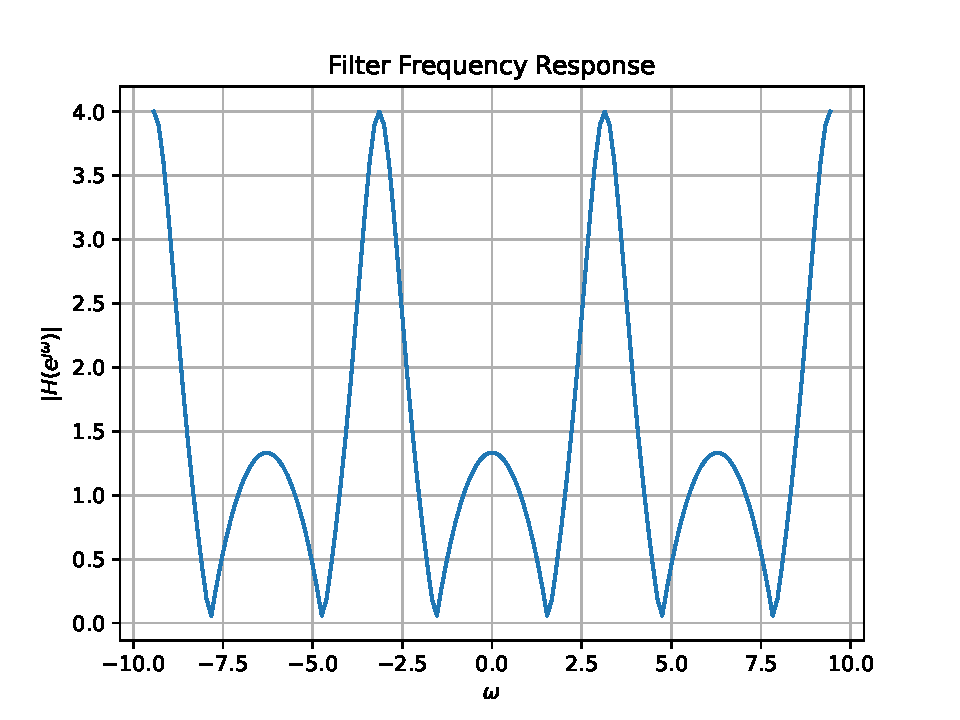
\includegraphics[width=\columnwidth]{./figs/dtft}
\caption{$\abs{H\brak{e^{\j\omega}}}$}
\label{fig:dtft}
\end{figure}
\begin{enumerate}
\item The Plot $\abs{H\brak{e^{\j\omega}}}$ is Symmetric about $\omega = 0$
\item The maximum and minimum values of the plot are 4 and 0 respectively 
\item Consider \eqref{eq:dtft},\\
The period of numerator is $\pi$ and the period of denominator is $2\pi$\\
$\therefore$ The period of $\abs{H\brak{e^{\j\omega}}}$ is $LCM(\pi,2\pi) = 2\pi$\\
i.e.,
\begin{align}
\abs{H\brak{e^{\j\brak{\omega + 2\pi}}}} &= \frac{4\abs{\cos\brak{\omega + 2\pi}}}{\sqrt{5+4\cos\brak{\omega + 2\pi}}}\\ &= \frac{4\abs{\cos{\omega}}}{\sqrt{5+4\cos{\omega}}}\\ \abs{H\brak{e^{\j\brak{\omega + 2\pi}}}} &= \abs{H\brak{e^{\j\omega}}}
\end{align}
$\Rightarrow$ it is Periodic with a period of $2\pi$
\end{enumerate}
\item Express $h(n)$ in terms of $H\brak{e^{\j \omega}}$.\\
\solution 
\begin{align}
H\brak{e^{\j\omega}} &= \sum_{n=-\infty}^{\infty}h(n)e^{-\j \omega n}
\end{align}
Multiply both sides with $e^{\j \omega k}$ and integrate from $-\pi$ to $\pi$
\begin{align}
\int_{-\pi}^{\pi}H\brak{e^{\j\omega}}e^{\j \omega k} d\omega &= \sum_{n=-\infty}^{\infty}h(n)\int_{-\pi}^{\pi}e^{-\j \omega n}e^{\j \omega k} d\omega\\ &= \sum_{n=-\infty}^{\infty}h(n)\int_{-\pi}^{\pi}e^{-\j \omega\brak{n-k}} d\omega\\ &= h(k)2\pi
\end{align}
Since,
\begin{align}
\int_{-\pi}^{\pi}e^{-\j\omega(n - k)}d\omega =
	\begin{cases}
		2\pi & n = k \\
		0 & \textrm{otherwise}
	\end{cases}
\end{align}
\begin{align}
\therefore h(n) &= \frac{1}{2\pi}\int_{-\pi}^{\pi}H\brak{e^{\j\omega}}e^{\j \omega n} d\omega
\end{align}
\end{enumerate}
\section{Impulse Response}
\begin{enumerate}[label=\thesection.\arabic*]
	\item Using long division, 
find
		\begin{align}
			h(n), \quad n < 5
		\end{align}
		for H(z) in 
		\eqref{eq:freq_resp}.\\
\solution From \eqref{eq:freq_resp}, we have\\
\begin{align}
H(z) = \frac{1 + z^{-2}}{1 + \frac{1}{2}z^{-1}}
\end{align}
Substitute $z^{-1} = x$ to perform long division
\polylongdiv{1 + x^2}{1 + \frac{1}{2}x}\\
From above division we can write,
\begin{align}
1+z^{-2} &= (1+\frac{1}{2}z^{-1})(2z^{-1}-4) + 5\\
\frac{1+z^{-2}}{1+\frac{1}{2}z^{-1}} &= 2z^{-1}-4 + \frac{5}{1+\frac{1}{2}z^{-1}}
\end{align}
From \eqref{eq:freq_resp}, we can write
\begin{align}
H(z) &= -4 + 2z^{-1} + \frac{5}{1 + \frac{1}{2}z^{-1}} \\
&= -4 + 2z^{-1} + 5\sum_{n = 0}^{\infty}\brak{-\frac{1}{2}}^nz^{-n} \\
&= 1 - \frac{1}{2}z^{-1} + 5\sum_{n = 2}^{\infty}\brak{-\frac{1}{2}}^nz^{-n} \\
&= \sum_{n = 0}^{\infty}\brak{-\frac{1}{2}}^nz^{-n} + 4\sum_{n = 2}^{\infty}\brak{-\frac{1}{2}}^nz^{-n} \\
&= \sum_{n = -\infty}^{\infty}u(n)\brak{-\frac{1}{2}}^nz^{-n} + \nonumber \\
&\sum_{n = -\infty}^{\infty}u(n - 2)\brak{-\frac{1}{2}}^{n - 2}z^{-n}
\end{align}
Therefore, from \eqref{eq:z_trans}, 
\begin{align}
	h(n) = \brak{-\frac{1}{2}}^{n}u(n) + \brak{-\frac{1}{2}}^{n-2}u(n-2)
\end{align}
\item \label{prob:impulse_resp}
Find an expression for $h(n)$ using $H(z)$,\\ given that 
%in Problem \ref{eq:ztransab} and \eqref{eq:anun}, given that
\begin{equation}
\label{eq:impulse_resp}
h(n) \ztrans H(z)
\end{equation}
and there is a one to one relationship between $h(n)$ and $H(z)$.\\
$h(n)$ is known as the {\em impulse response} of the
system defined by \eqref{eq:iir_filter}.\\
\solution From \eqref{eq:freq_resp},
\begin{equation}
\label{eq:hz}
H(z) = \frac{1}{1 + \frac{1}{2}z^{-1}} + \frac{ z^{-2}}{1 + \frac{1}{2}z^{-1}}
\end{equation}
From \eqref{eq:anun},
\begin{align}
&\frac{1}{1 + \frac12 z^{-1}} \ztrans \brak{-\frac12}^n u(n) \quad \abs{z} > \frac12 \\
&\frac{z^{-2}}{1 + \frac12 z^{-1}} \ztrans \brak{-\frac12}^{n-2} u(n-2) \quad \abs{z} > \frac12\\
\Rightarrow & H(z) \ztrans \brak{-\frac12}^n u(n) + \brak{-\frac12}^{n-2} u(n-2) \quad \abs{z} > \frac12\\
\end{align}
(Since Z-transform is a linear operator)
\begin{align}
\therefore h(n) = \brak{-\frac12}^n u(n) + \brak{-\frac12}^{n-2} u(n-2) 
\end{align}
From \eqref{eq:hz},Consider the first part:
\begin{align}
\frac{1}{1 + \frac{1}{2}z^{-1}} &= \sum_{n=0}^{\infty}\brak{-\frac{1}{2}}^n z^n
\end{align}
This sum converges when $\abs{z}>\frac{1}{2}$\\
$\Rightarrow$ ROC is $\abs{z}>\frac{1}{2} $
\begin{align}
\frac{1}{1 + \frac{1}{2}z^{-1}} &= \frac{2z}{1+2z}\\ &= \sum_{n=-\infty}^{-1}\brak{2z}^{-n}
\end{align}
This sum converges when $\abs{z}<\frac{1}{2}$\\
$\Rightarrow$ ROC is $\abs{z}<\frac{1}{2} $\\
Therefore, ROC of $H(z)$ will be
\begin{align}
\abs{z} \neq \frac{1}{2}
\end{align}
\item Sketch $h(n)$. Is it bounded? Convergent? 
\solution The following code plots Fig. \ref{fig:hn}.
\begin{lstlisting}
https://github.com/JBA-12/EE3900/blob/main/A1/codes/5.3.py
\end{lstlisting}
and run the code using the following command
\begin{lstlisting}
python3 5.3.py
\end{lstlisting}
\begin{figure}[!ht]
\centering
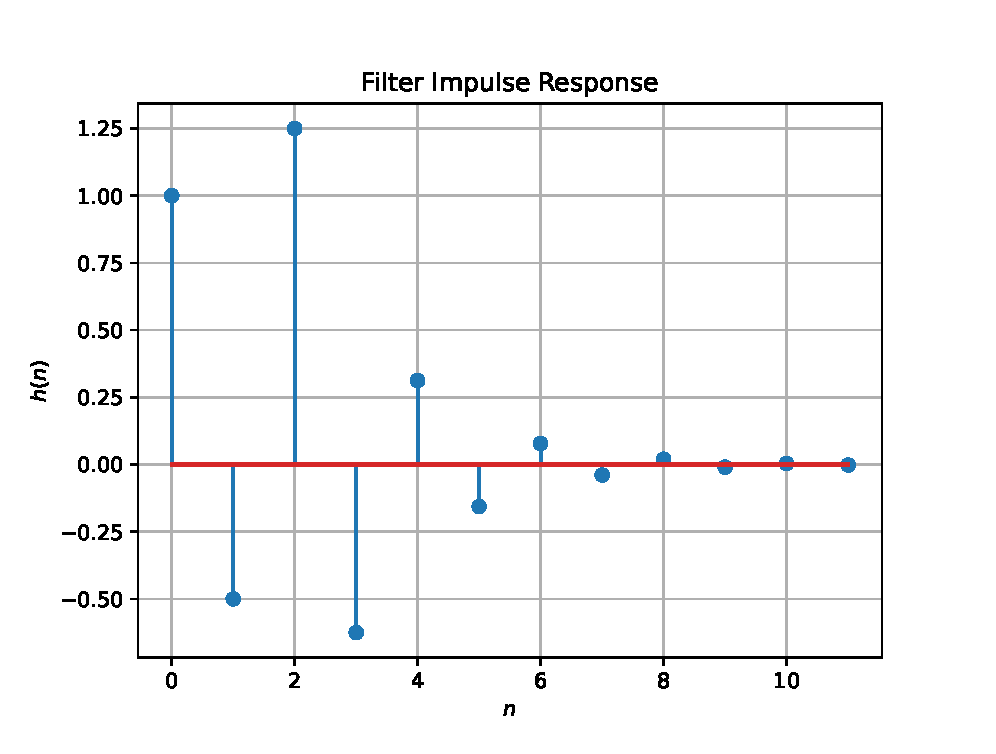
\includegraphics[width=\columnwidth]{./figs/hn}
\caption{$h(n)$ as the inverse of $H(z)$}
\label{fig:hn}
\end{figure}
From the plot, we can conclude that it is convergent to 0 \\
$\Rightarrow$ It is bounded as well.
%
\item Convergent? Justify using the ratio test.\\
\solution Using the ratio test for convergence
\begin{align}
\lim_{n \to \infty} \abs{\frac{h(n+1)}{h(n)}} &= \lim_{n \to \infty} \abs{\frac{\brak{-\frac{1}{2}}^{n-1} \brak{1+\frac{1}{4}}}{\brak{-\frac{1}{2}}^{n-2}\brak{1+\frac{1}{4}}}}\\ &= \lim_{n \to \infty} \abs{-\frac{1}{2}}\\ &= \frac{1}{2}<1
\end{align}
$\therefore$ h(n) is Convergent.
\item The system with $h(n)$ is defined to be stable if
\begin{equation}
\sum_{n=-\infty}^{\infty}h(n) < \infty
\end{equation}
Is the system defined by \eqref{eq:iir_filter} stable for the impulse response in \eqref{eq:impulse_resp}?\\
\solution From 5.2,
\begin{align}
\sum_{n=-\infty}^{\infty}h(n) &= \sum_{n=-\infty}^{\infty}\brak{-\frac{1}{2}}^{n}u(n) + \sum_{n=-\infty}^{\infty}\brak{-\frac{1}{2}}^{n-2}u(n-2)\\ &= \sum_{n=0}^{\infty}\brak{-\frac{1}{2}}^{n} + \sum_{n=0}^{\infty}\brak{-\frac{1}{2}}^{n-2}u(n-2)\\ &= \frac{1}{1-\brak{\frac{-1}{2}}} + \frac{1}{1-\brak{\frac{-1}{2}}}\\ &= \frac{4}{3} < \infty
\end{align}
using the fomula for the sum of an infinite geometric progression\\\\
$\therefore$ The system is stable.
\item Verify the above result using a python code.\\
\solution The following code verifies whether the given system is stable or not
\begin{lstlisting}
https://github.com/JBA-12/EE3900/blob/main/A1/codes/5.6.py
\end{lstlisting}
run the code using the following command
\begin{lstlisting}
python3 5.6.py
\end{lstlisting}
\item 
Compute and sketch $h(n)$ using 
\begin{equation}
\label{eq:iir_filter_h}
h(n) + \frac{1}{2}h(n-1) = \delta(n) + \delta(n-2), 
\end{equation}
%
This is the definition of $h(n)$.
\\
\solution The following code plots Fig. \ref{fig:hndef}. Note that this is the same as Fig. \ref{fig:hn}. 
%
\begin{lstlisting}
https://github.com/JBA-12/EE3900/blob/main/A1/codes/5.7.py
\end{lstlisting}
run the code using the following command
\begin{lstlisting}
python3 5.7.py
\end{lstlisting}
\begin{figure}[!ht]
\centering
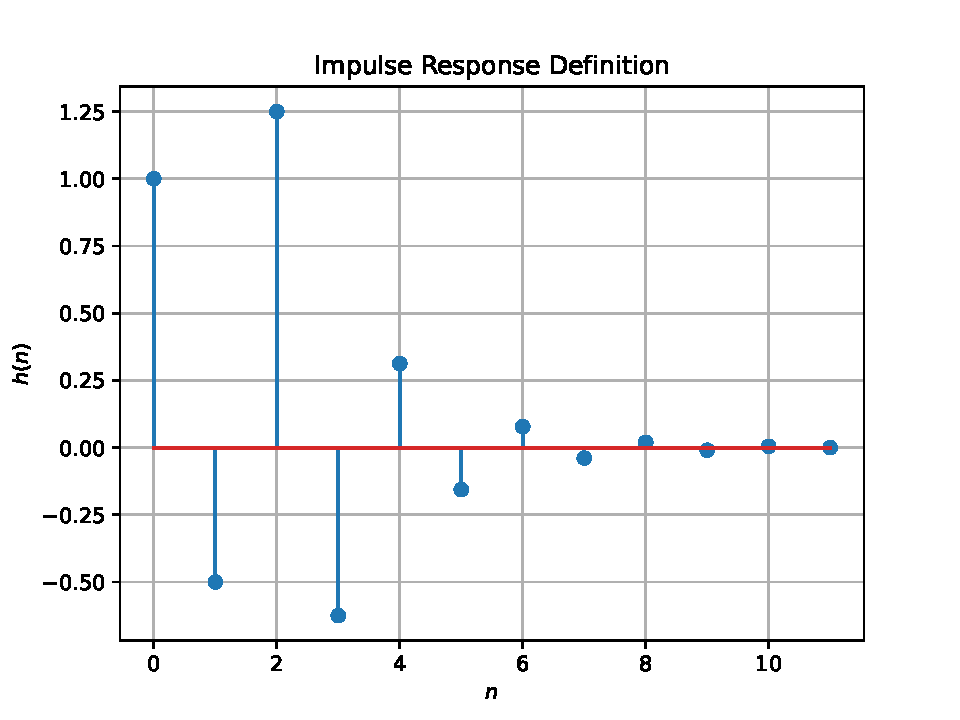
\includegraphics[width=\columnwidth]{./figs/hndef}
\caption{$h(n)$ from the definition}
\label{fig:hndef}
\end{figure}
%
\item Compute 
%
\begin{equation}
\label{eq:convolution}
y(n) = x(n)*h(n) = \sum_{k=-\infty}^{\infty}x(k)h(n-k)
\end{equation}
%
Comment. The operation in \eqref{eq:convolution} is known as
{\em convolution}.
%
\\
\solution 
\begin{align}
x(n)*h(n) &= \sum_{k=-\infty}^{\infty}x(k)h(n-k)\\ &= \sum_{k=0}^{5}x(k)h(n-k)
\end{align}
The following code plots Fig. \ref{fig:ynconv}.
%
\begin{lstlisting}
https://github.com/JBA-12/EE3900/blob/main/A1/codes/5.8.py
\end{lstlisting}
run the code using the following command
\begin{lstlisting}
python3 5.8.py
\end{lstlisting}
\begin{figure}[!htbp]
\centering
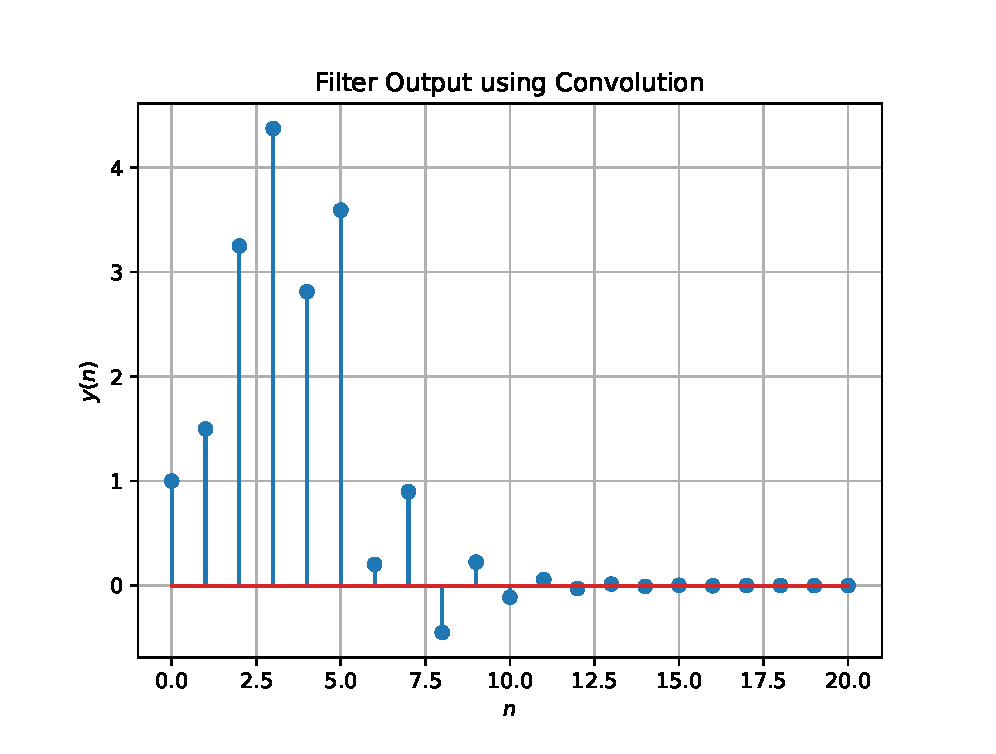
\includegraphics[width=\columnwidth]{./figs/ynconv}
\caption{$y(n)$ from the definition of convolution}
\label{fig:ynconv}
\end{figure}
This plot is same as y(n) in Fig. \ref{fig:xnyn}\\\\
Therefore,
\begin{align}
y(n) = x(n) * h(n)
\end{align}
\item Express the above convolution using a Teoplitz matrix.\\
\solution From \eqref{def:xn},we can write
\begin{align}
\vec{x} = \myvec{1 \\ 2 \\ 3 \\ 4 \\ 2 \\ 1} \qquad
\vec{h} = \myvec{1 \\ -0.5 \\ 1.25 \\ -0.62 \\ 0.31 \\ -0.16}
\end{align}
Their convolution is given by the product of the following Toeplitz matrix $\vec{T}$
\begin{align}
		&\myvec{
			1 & 0 & 0 & 0 & 0 & 0 \\
			-0.5 & 1 & 0 & 0 & 0 & 0 \\
			1.25 & -0.5 & 1 & 0 & 0 & 0 \\
			-0.62 & 1.25 & -0.5 & 1 & 0 & 0 \\
			0.31 & -0.62 & 1.25 & -0.5 & 1 & 0 \\
			-0.16 & 0.31 & -0.62 & 1.25 & -0.5 & 1 \\
			0 & -0.16 & 0.31 & -0.62 & 1.25 & -0.5 \\
			0 & 0 & -0.16 & 0.31 & -0.62 & 1.25 \\
			0 & 0 & 0 & -0.16 & 0.31 & -0.62 \\
			0 & 0 & 0 & 0 & -0.16 & 0.31 \\
			0 & 0 & 0 & 0 & 0 & -0.16 \\
		} 
\end{align}
\begin{align}
&\vec{y} = \vec{x} \circledast \vec{h} = \vec{Tx} = \myvec{1 \\ 1.5 \\ 3.25 \\ 4.38 \\ 2.81 \\ 3.59 \\ 0.12 \\ 0.78 \\ -0.62 \\ 0 \\ -0.16}
\end{align}
The following python code computes the convolution using Teoplitz matrix.
\begin{lstlisting}
https://github.com/JBA-12/EE3900/blob/main/A1/codes/5.9.py
\end{lstlisting}
run the code using the following command
\begin{lstlisting}
python3 5.9.py
\end{lstlisting}
\begin{figure}[!htbp]
\centering
\includegraphics[width=\columnwidth]{./figs/5.9}
\caption{$y(n)$ from the definition of convolution using Teoplitz matrix}
\label{fig:ynconv}
\end{figure}
\item Show that
\begin{equation}
y(n) =  \sum_{k=-\infty}^{\infty}x(n-k)h(k)
\end{equation}
\solution From \eqref{eq:convolution} we know that,
\begin{align}
y(n) = x(n)*h(n) &= \sum_{k=-\infty}^{\infty}x(k)h(n-k)
\end{align}
Substitute k = n-i
\begin{align}
\sum_{k=-\infty}^{\infty}x(k)h(n-k) &= \sum_{n-i=-\infty}^{\infty}x(n-i)h(n-(n-i))\\ &= \sum_{i=\infty}^{-\infty}x(n-i)h(i)\\ &= \sum_{i=-\infty}^{\infty}x(n-i)h(i)
\end{align}
Since, the order of limit doesn't matter in case of summation.Therefore, now we have
\begin{align}
\sum_{k=-\infty}^{\infty}x(k)h(n-k) = \sum_{k=-\infty}^{\infty}x(n-k)h(k)
\end{align}
from \eqref{eq:convolution}
\begin{align}
\therefore y(n) = \sum_{k=-\infty}^{\infty}x(n-k)h(k)
\end{align}
\end{enumerate}
\section{DFT }
\begin{enumerate}[label=\thesection.\arabic*]
\item
Compute
\begin{equation}
X(k) \define \sum _{n=0}^{N-1}x(n) e^{-\j2\pi kn/N}, \quad k = 0,1,\dots, N-1
\end{equation}
and $H(k)$ using $h(n)$.\\
\solution The following code plots Fig. \ref{fig:dft}.
\begin{lstlisting}
https://github.com/JBA-12/EE3900/blob/main/A1/codes/6.1.py
\end{lstlisting}
and run the python code using the following command
\begin{lstlisting}
python3 6.1.py
\end{lstlisting}
\begin{figure}[!htbp]
\centering
\includegraphics[width=\columnwidth]{./figs/dft}
\caption{Plot of real part of Discrete Fourier Transforms of x(n) and h(n)}
\label{fig:dft}
\end{figure}
\item Compute 
\begin{equation}
Y(k) = X(k)H(k)
\end{equation}
\solution The following code plots Fig. \ref{fig:Y_k}.
\begin{lstlisting}
https://github.com/JBA-12/EE3900/blob/main/A1/codes6.2.py
\end{lstlisting}
and run the code using the following command
\begin{lstlisting}
python3 6.2.py
\end{lstlisting}
\begin{figure}[!htbp]
\centering
\includegraphics[width=\columnwidth]{./figs/Y_k}
\caption{Y(k) as product of X(k) and H(k)}
\label{fig:Y_k}
\end{figure}
\item Compute
\begin{equation}
 y\brak{n}={\frac {1}{N}}\sum _{k=0}^{N-1}Y\brak{k}\cdot e^{\j 2\pi kn/N},\quad n = 0,1,\dots, N-1
\end{equation}
\\
\solution The following code plots Fig. \ref{fig:yndft_dif}.
\begin{lstlisting}
https://github.com/JBA-12/EE3900/blob/main/A1/codes/6.3.py
\end{lstlisting}
and run the code using the following command 
\begin{lstlisting}
python3 6.3.py
\end{lstlisting}
\begin{figure}[!htbp]
\centering
\includegraphics[width=\columnwidth]{./figs/yndft_dif}
\caption{$y(n)$ using IDFT and Difference Equation}
\label{fig:yndft_dif}
\end{figure}
\item Repeat the previous exercise by computing $X(k), H(k)$ and $y(n)$ through FFT and 
IFFT.
\solution The following code plots Fig. \ref{fig:yn_ifft}.
\begin{lstlisting}
https://github.com/JBA-12/EE3900/blob/main/A1/codes/6.4.py
\end{lstlisting}
and run the code using the following command 
\begin{lstlisting}
python3 6.4.py
\end{lstlisting}
\begin{figure}[!htbp]
\centering
\includegraphics[width=\columnwidth]{./figs/yn_ifft}
\caption{The plot of y(n) using IFFT}
\label{fig:yn_ifft}
\end{figure}
\item Wherever possible, express all the above equations as matrix equations.
\solution
  \begin{align}
		\vec{x} &= \myvec{x_0 & x_1	 & \cdots & x_{N-1}}^\top \\
		\vec{h} &= \myvec{x_0 & x_1	 & \cdots & x_{N-1}}^\top \\
		\vec{y} &= \vec{x} \circledast \vec{h} \\
		\myvec{y_1 \\ y_2 \\ \vdots \\ y_{2N - 1}} &= \myvec{
			h_0 & 0 & 0 & \cdots & 0 \\
			h_1 & h_0 & 0 & \cdots & 0 \\
			h_2 & h_1 & h_0 & \cdots & 0 \\
			\vdots & \vdots & \vdots & \ddots & \vdots \\
			h_{N-1} & h_{N-2} & h_{N-3} & \cdots & h_0 \\
			0 & h_{N-1} & h_{N-2} & \cdots & h_1 \\
			0 & 0 & h_{N-1} & \cdots & h_2 \\
			\vdots & \vdots & \vdots & \ddots & \vdots \\
			0 & 0 & 0 & \cdots & h_{N-1}
		}		
		\myvec{x_1\\x_2\\ \vdots \\x_N}
	\end{align}
The convolution can be written using a Toeplitz matrix. 
Consider the DFT matrix
\begin{align}
\vec{W} = \myvec{1 & 1 & 1 & 1 & \cdots & 1 \\
          1 & \omega & \omega^2 & \omega^3 & \cdots & \omega^{N-1} \\
			1 & \omega^2 & \omega^4 & \omega^6 & \cdots &
\omega^{2(N-1)} \\
			1 & \omega^3 & \omega^6 & \omega^9 & \cdots & \omega^{3(N-1)} \\
			\vdots & \vdots & \vdots & \vdots & \ddots & \vdots \\ 
			1 & \omega^{N-1} & \omega^{2(N-1)} & \omega^{3(N-1)} & \cdots & \omega^{(N-1)(N-1)}
		}
\end{align}
where $\omega = e^{-\j 2\pi/N}$ is the $N^{\mathrm{th}}$ root of unity
Then the discrete Fourier transforms of $\vec{x}$ and $\vec{h}$ are given by
	\begin{align}
		\vec{X} &= \vec{W} \vec{x} \\
		\vec{H} &= \vec{W} \vec{h}
	\end{align}
	
	$\vec{Y}$ is then given by
	\begin{equation}
		\vec{Y} = \vec{X} \circ \vec{H}
	\end{equation}
where $\circ$ denotes the Hadamard product (element-wise multiplication)
	
But $\vec{Y}$ is the discrete Fourier transform of the filter output $\vec{y}$
	\begin{equation}
		\vec{Y} = \vec{W} \vec{y}
	\end{equation}
	
	Thus,
	\begin{align}
		\vec{W} \vec{y} &= \vec{X} \circ \vec{H} \\
		\implies \vec{y} &= \vec{W}^{-1} \brak{\vec{X} \circ \vec{H}} \\
		&= \vec{W}^{-1} \brak{\vec{W} \vec{x} \circ \vec{W} \vec{h}}
	\end{align}
	This is the inverse discrete Fourier transform of $\vec{Y}$
\item Verify the above equations by generating the DFT matrix in python.
\end{enumerate}
\section{FFT}
% \subsection{Definitions}
\begin{enumerate}[label=\arabic*.,ref=\thesection.\theenumi]
\numberwithin{equation}{section}
    \item The DFT of $x(n)$ is given by
    \begin{align}
        X(k) \triangleq \sum_{n=0}^{N-1} x(n) e^{-j 2 \pi k n / N}, \quad k=0,1, \ldots, N-1
    \end{align}
\item Let 
	\begin{align}
W_{N} = e^{-j2\pi/N} 
	\end{align}
		Then the $N$-point {\em DFT matrix} is defined as 
	\begin{align}
		\vec{F}_{N} = \sbrak{W_{N}^{mn}}, \quad 0 \le m,n \le N-1 
	\end{align}
	where $W_{N}^{mn}$ are the elements of $\vec{F}_{N}$.
\item Let 
	\begin{align}
		\vec{I}_4 = \myvec{\vec{e}_4^{1} &\vec{e}_4^{2} &\vec{e}_4^{3} &\vec{e}_4^{4} }
	\end{align}
		be the $4\times 4$ identity matrix.  Then the 4 point {\em DFT permutation matrix} is defined as 
	\begin{align}
		\vec{P}_4 = \myvec{\vec{e}_4^{1} &\vec{e}_4^{3} &\vec{e}_4^{2} &\vec{e}_4^{4} }
	\end{align}
\item The 4 point {\em DFT diagonal matrix} is defined as 
	\begin{align}
		\vec{D}_4 = diag\myvec{W_{8}^{0} & W_{8}^{1} & W_{8}^{2} & W_{8}^{3}}
	\end{align}
\item Show that 
\begin{equation}
    W_{N}^{2}=W_{N/2}
\end{equation}
\solution 
\begin{align}
W_{N}^{2} &= e^{-j2\pi/N} e^{-j2\pi/N}\\ &= e^{2\brak{-j2\pi/N}}\\ &= e^{-j2\pi/\frac{N}{2}}\\ &= W_{N/2}
\end{align}
%    \item Find $\vec{P}_6$.
%    \item Find $\vec{D}_3$.
    \item Show that 
\begin{equation}
	\vec{F}_{4}=
\begin{bmatrix}
	\vec{I}_{2} & \vec{D}_{2} \\
\vec{I}_{2} & -\vec{D}_{2}
\end{bmatrix}
\begin{bmatrix}
\vec{F}_{2} & 0 \\
0 & \vec{F}_{2}
\end{bmatrix}
\vec{P}_{4}
\end{equation}
\solution 
\begin{align}
&\mymat{\vec{I}_2 & \vec{D}_2 \\ \vec{I}_2 & -\vec{D}_2}\mymat{\vec{F}_2 & 0 \\ 0 & \vec{F}_2} \\= &\mymat{\vec{F}_2 & \vec{D}_2\vec{F}_2 \\ \vec{F}_2 & -\vec{D}_2\vec{F}_2}  \\= &\mymat{\myvec{1&1\\1&-1} & \myvec{1&0\\0&-\j}\myvec{1&1\\1&-1} \\ \myvec{1&1\\1&-1} & - \myvec{1&0\\0&-\j}\myvec{1&1\\1&-1}} \\= &\mymat{1 & 1 & 1 & 1 \\ 1 & -1 & -\j & \j \\ 1 & 1 & -1 & -1 \\ 1 & -1 & \j & -\j}
\end{align}	
Now
\begin{align}
&\mymat{\vec{I}_2 & \vec{D}_2 \\ \vec{I}_2 & -\vec{D}_2}\mymat{\vec{F}_2 & 0 \\ 0 & \vec{F}_2} \vec{P}_4 \\= &\mymat{1 & 1 & 1 & 1 \\ 1 & -1 & -\j & \j \\ 1 & 1 & -1 & -1 \\ 1 & -1 & \j & -\j} \mymat{1 & 0 & 0 & 0 \\ 0 & 0 & 1 & 0 \\ 0 & 1 & 0 & 0 \\ 0 & 0 & 0 & 1} \\= &\mymat{1 & 1 & 1 & 1 \\ 1 & -\j & -1 & \j \\ 1 & -1 & 1 & -1 \\ 1 & \j & -1 & -\j} \\= &\mymat{W_4^0 & W_4^0 & W_4^0 & W_4^0 \\ W_4^0 & W_4^1 & W_4^2 & W_4^3 \\ W_4^0 & W_4^2 & W_4^4 & W_4^6 \\ W_4^0 & W_4^3 & W_4^6 & W_4^9} \\= &~\vec{F}_4
\end{align}
since,
	\begin{align}
		W_4^0 &= 1 \\
		W_4^1 &= e^{-\j\frac{\pi}{2}} = -\j \\
		W_4^2 &= e^{-\j\pi} = -1 \\
		W_4^3 &= e^{-\j\frac{3\pi}{2}} = \j \\
		W_4^n &= W_4^{n - 4} &&\forall n \ge 4
	\end{align}	
\item Show that 
\begin{equation}
\vec{F}_{N}=
\begin{bmatrix}
\vec{I}_{N/2} & \vec{D}_{N/2} \\
\vec{I}_{N/2} & -\vec{D}_{N/2}
\end{bmatrix}
\begin{bmatrix}
\vec{F}_{N/2} & 0 \\
0 & \vec{F}_{N/2}
\end{bmatrix}
\vec{P}_{N}
\end{equation}
\solution
\begin{align}
&\mymat{\vec{I}_{N/2} & \vec{D}_{N/2} \\ \vec{I}_{N/2} & -\vec{D}_{N/2}} \mymat{\vec{F}_{N/2} & 0 \\ 0 & \vec{F}_{N/2}}  \\= &\mymat{\vec{F}_{N/2} & \vec{D}_{N/2}\vec{F}_{N/2} \\ \vec{F}_{N/2} & -\vec{D}_{N/2}\vec{F}_{N/2}}
\end{align}
Now
\begin{align}
&\vec{D}_{N/2}\vec{F}_{N/2} \\&= \mymat{W_N^0 & \cdots & 0 \\ \vdots & \ddots & \vdots \\ 0 & \cdots & W_N^{N/2-1}} \mymat{W_{N/2}^0 & \cdots & W_{N/2}^0 \\ \vdots & \ddots & \vdots \\ W_{N/2}^0 & \cdots & W_{N/2}^{(N/2 - 1)^2}} \\&= \mymat{W_N^0 W_{N/2}^0 & \cdots & W_N^0 W_{N/2}^0 \\ \vdots & \ddots & \vdots \\ W_N^{N/2-1} W_{N/2}^0 & \cdots & W_N^{N/2-1} W_{N/2}^{(N/2 - 1)^2}} 
\end{align}
Thus
\begin{align}
\brak{\vec{D}_{N/2}\vec{F}_{N/2}}_{ij} &= W_N^i W_{N/2}^{ij} \\
&= W_N^i W_N^{2ij} \\&= W_N^{i(2j + 1)}
\end{align}
where $i, j = 0, \ldots, N/2 - 1$
Therefore, $\vec{D}_{N/2}\vec{F}_{N/2}$ forms the first $N/2$ rows of the odd-indexed columns of $\vec{F}_N$
\begin{align}
W_N^{(i + N/2)(2j + 1)} &= \exp\brak{-\j \frac{2\pi}{N} (2j + 1)\brak{i + \frac{N}{2}}} \\&= \exp\brak{-\j \brak{\frac{2\pi}{N} (2j + 1)i + (2j + 1)\pi}} \\&= -\exp\brak{-\j \frac{2\pi}{N} (2j + 1)i} \\
&= -W_N^{i(2j + 1)}
\end{align}
Thus, the remaining $N/2$ rows will be the negatives of the first $N/2$ rows
\begin{align}
\brak{\vec{F}_{N/2}}_{ij} &= W_{N/2}^{ij} \\&= W_N^{i(2j)}
\end{align}
where $i, j = 0, \ldots, N/2 - 1$
Therefore, $\vec{F}_{N/2}$ forms the first $N/2$ rows of the even-indexed columns of $\vec{F}_N$
\begin{align}
W_N^{(i + N/2)(2j)} &= \exp\brak{-\j \frac{2\pi}{N} (2j)\brak{i + \frac{N}{2}}} \\&= \exp\brak{-\j \brak{\frac{2\pi}{N} (2j)i + (2j)\pi}} \\&= \exp\brak{-\j \frac{2\pi}{N} (2j)i} \\&= W_N^{i(2j)}
\end{align}
Thus, the remaining $N/2$ rows will be the same as the first $N/2$ rows
Therefore
\begin{align}
\mymat{\vec{F}_{N/2} & \vec{D}_{N/2}\vec{F}_{N/2} \\ \vec{F}_{N/2} & -\vec{D}_{N/2}\vec{F}_{N/2}} = \vec{F}_N \vec{P}_N
\end{align}
where 
\begin{align}
\vec{P}_N = \myvec{\vec{e}_N^1 & \vec{e}_N^3 & \cdots & \vec{e}_N^{N-1} & \vec{e}_N^2 & \vec{e}_N^4 & \cdots & \vec{e}_N^N}
\end{align}
Hence
\begin{align}
\mymat{\vec{F}_{N/2} & \vec{D}_{N/2}\vec{F}_{N/2} \\ \vec{F}_{N/2} & -\vec{D}_{N/2}\vec{F}_{N/2}} \vec{P}_N = \vec{F}_N \vec{P}_N^2 = \vec{F}_N \\\therefore \vec{F}_N = \mymat{\vec{I}_{N/2} & \vec{D}_{N/2} \\ \vec{I}_{N/2} & -\vec{D}_{N/2}} \mymat{\vec{F}_{N/2} & 0 \\ 0 & \vec{F}_{N/2}} \vec{P}_N
\end{align}
for even $N$
\item Find 
    \begin{align}
	     \vec{P}_4 \vec{x}
    \end{align}
\solution Let $\vec{x} = \myvec{x(0) & x(1) & x(2) & x(3)}^\top$
\begin{align}
\vec{P}_4 \vec{x} &= \mymat{1 & 0 & 0 & 0 \\ 0 & 0 & 1 & 0 \\ 0 & 1 & 0 & 0 \\ 0 & 0 & 0 & 1} \mymat{x(0) \\ x(1) \\ x(2) \\ x(3)} \\
&= \mymat{x(0) \\ x(2) \\ x(1) \\ x(3)}
\end{align}
\item Show that 
    \begin{align}
	    \vec{X} = \vec{F}_N \vec{x}
	    \label{eq:dft-mat-def}
    \end{align}
		where $\vec{x}, \vec{X}$ are the vector representations of $x(n), X(k)$ respectively.
\solution 
\begin{align}
X(k) &= \sum_{n=0}^{N-1} x(n) e^{-j 2 \pi k n / N}, \quad k=0,1, \ldots, N-1 \\\implies \vec{X} &= \mymat{\sum_{n=0}^{N-1} x(n) e^{-j 2 \pi  n (0) / N} \\ \vdots \\ \sum_{n=0}^{N-1} x(n) e^{-j 2 \pi  n (N-1) / N}} \\&= \mymat{x(0) + \cdots + x(N-1) \\ \vdots \\ x(0) + \cdots + x(N-1) e^{-j 2 \pi (N-1)^2 / N}} 
\end{align}
\begin{align}
\vec{X} &= x(0) \mymat{1 \\ \vdots \\ 1} + \cdots + x(N-1)\mymat{1 \\ \vdots \\ e^{-j 2 \pi (N-1)^2 / N}} \\&= \mymat{1 & \cdots & 1 \\ \vdots & \ddots & \vdots \\ 1 & \cdots & e^{-j 2 \pi (N-1)^2 / N}} \mymat{x(0) \\ \vdots \\ x(N-1)} \\&= \vec{F}_N \vec{x}
\end{align}
\item Derive the following Step-by-step visualisation  of
8-point FFTs into 4-point FFTs and so on
\begin{equation}
\begin{bmatrix}
X(0) \\ 
X(1) \\ 
X(2) \\ 
X(3)
\end{bmatrix}
=
\begin{bmatrix}
X_{1}(0) \\ 
X_{1}(1)\\ 
X_{1}(2)\\
X_{1}(3)\\
\end{bmatrix}
+
\begin{bmatrix}
W^{0}_{8} & 0 & 0 & 0\\
0 & W^{1}_{8} & 0 & 0\\
0 & 0 & W^{2}_{8} & 0\\
0 & 0 & 0 & W^{3}_{8}
\end{bmatrix}
\begin{bmatrix}
X_{2}(0) \\ 
X_{2}(1) \\ 
X_{2}(2) \\
X_{2}(3)
\end{bmatrix}
\end{equation}
\begin{equation}
\begin{bmatrix}
X(4) \\ 
X(5) \\ 
X(6) \\ 
X(7)
\end{bmatrix}
=
\begin{bmatrix}
X_{1}(0) \\ 
X_{1}(1)\\ 
X_{1}(2)\\
X_{1}(3)\\
\end{bmatrix}
-
\begin{bmatrix}
W^{0}_{8} & 0 & 0 & 0\\
0 & W^{1}_{8} & 0 & 0\\
0 & 0 & W^{2}_{8} & 0\\
0 & 0 & 0 & W^{3}_{8}
\end{bmatrix}
\begin{bmatrix}
X_{2}(0) \\ 
X_{2}(1) \\ 
X_{2}(2) \\
X_{2}(3)
\end{bmatrix}
\end{equation}
4-point FFTs into 2-point FFTs
\begin{equation}
\begin{bmatrix}
X_{1}(0) \\ 
X_{1}(1)\\ 
\end{bmatrix}
=
\begin{bmatrix}
X_{3}(0) \\ 
X_{3}(1)\\ 
\end{bmatrix}
+
\begin{bmatrix}
W^{0}_{4} & 0\\
0 & W^{1}_{4}
\end{bmatrix}
\begin{bmatrix}
X_{4}(0) \\ 
X_{4}(1) \\ 
\end{bmatrix}
\end{equation}
\begin{equation}
\begin{bmatrix}
X_{1}(2) \\ 
X_{1}(3)\\ 
\end{bmatrix}
=
\begin{bmatrix}
X_{3}(0) \\ 
X_{3}(1)\\ 
\end{bmatrix}
-
\begin{bmatrix}
W^{0}_{4} & 0\\
0 & W^{1}_{4}
\end{bmatrix}
\begin{bmatrix}
X_{4}(0) \\ 
X_{4}(1) \\ 
\end{bmatrix}
\end{equation}
\begin{equation}
\begin{bmatrix}
X_{2}(0) \\ 
X_{2}(1)\\ 
\end{bmatrix}
=
\begin{bmatrix}
X_{5}(0) \\ 
X_{5}(1)\\ 
\end{bmatrix}
+
\begin{bmatrix}
W^{0}_{4} & 0\\
0 & W^{1}_{4}
\end{bmatrix}
\begin{bmatrix}
X_{6}(0) \\ 
X_{6}(1) \\ 
\end{bmatrix}
\end{equation}
\begin{equation}
\begin{bmatrix}
X_{2}(2) \\ 
X_{2}(3)\\ 
\end{bmatrix}
=
\begin{bmatrix}
X_{5}(0) \\ 
X_{5}(1)\\ 
\end{bmatrix}
-
\begin{bmatrix}
W^{0}_{4} & 0\\
0 & W^{1}_{4}
\end{bmatrix}
\begin{bmatrix}
X_{6}(0) \\ 
X_{6}(1) \\ 
\end{bmatrix}
\end{equation}
\begin{equation}
P_{8}
\begin{bmatrix}
x(0) \\ 
x(1) \\ 
x(2) \\ 
x(3) \\ 
x(4) \\ 
x(5) \\
x(6) \\
x(7)
\end{bmatrix}
 = 
\begin{bmatrix}
x(0) \\ 
x(2) \\ 
x(4) \\ 
x(6) \\
x(1) \\ 
x(3) \\ 
x(5) \\
x(7)
\end{bmatrix}
\end{equation}
\begin{equation}
P_{4}
\begin{bmatrix}
x(0) \\ 
x(2) \\ 
x(4) \\ 
x(6) \\
\end{bmatrix}
 = 
\begin{bmatrix}
x(0) \\ 
x(4) \\ 
x(2) \\
x(6)
\end{bmatrix}
\end{equation}
\begin{equation}
P_{4}
\begin{bmatrix}
x(1) \\ 
x(3) \\ 
x(5) \\
x(7)
\end{bmatrix}
 = 
\begin{bmatrix}
x(1) \\ 
x(5) \\ 
x(3) \\ 
x(7) \\
\end{bmatrix}
\end{equation}
Therefore,
\begin{equation}
\begin{bmatrix}
X_{3}(0) \\ 
X_{3}(1)\\ 
\end{bmatrix}
= F_{2}
\begin{bmatrix}
x(0) \\ 
x(4) \\ 
\end{bmatrix}
\end{equation}
\begin{equation}
\begin{bmatrix}
X_{4}(0) \\ 
X_{4}(1)\\ 
\end{bmatrix}
= F_{2}
\begin{bmatrix}
x(2) \\ 
x(6) \\ 
\end{bmatrix}
\end{equation}
\begin{equation}
\begin{bmatrix}
X_{5}(0) \\ 
X_{5}(1)\\ 
\end{bmatrix}
= F_{2}
\begin{bmatrix}
x(1) \\ 
x(5) \\ 
\end{bmatrix}
\end{equation}
\begin{equation}
\begin{bmatrix}
X_{6}(0) \\ 
X_{6}(1)\\ 
\end{bmatrix}
= F_{2}
\begin{bmatrix}
x(3) \\ 
x(7) \\ 
\end{bmatrix}
\end{equation}
\solution 
\begin{align}
        X(k) &= \sum_{n=0}^7 x(n) e^{-j 2 \pi k n / 8}, \quad k=0, \ldots, 7\\
        &= \sum_{n=0}^7 x(n) W_8^{kn} \\
        &= \sum_{n \text{ is even}}x(n) W_8^{kn} + \sum_{n \text{ is odd}}x(n) W_8^{kn} \\
        &= \sum_{m=0}^3 x(2m) W_8^{2km} + \sum_{m=0}^3 x(2m+1) W_8^{2km + k}
    \end{align}	
    
    Now substitute $W_8^2 = W_4$
    \begin{align}
    		X(k) = \sum_{m=0}^3 x(2m) W_4^{km} + W_8^k \sum_{m=0}^3 x(2m+1) W_4^{km}
    \end{align}
    
    Consider
    \begin{align}
    		x_1(n) = \cbrak{x(0), x(2), x(4), x(6)} \\
    		x_2(n) = \cbrak{x(1), x(3), x(5), x(7)}
    \end{align}
    
    Thus
    \begin{align}
    		X(k) = X_1(k) + W_8^k X_2(k) \qquad k = 0,\ldots,7
    \end{align}
    
    Now, $X_1(k)$ and $X_2(k)$ are $4$-point DFTs which means they are periodic with period $4$
    \begin{align}
    		X(k+4) &= X_1(k+4) + W_8^{k+4} X_2(k+4) \\
    		&= X_1(k) + e^{-\j 2\pi(k+4)/8} X_2(k) \\
    		&= X_1(k) + e^{-\j (2\pi k/8 + \pi)} X_2(k) \\
    		&= X_1(k) - e^{-\j 2\pi k/8 } X_2(k) \\
    		&= X_1(k) - W_8^k X_2(k)
    \end{align}
    
    Therefore, for $k=0,1,2,3$
    \begin{align}
    		X(k) = X_1(k) + W_8^k X_2(k)  \\
    		X(k+4) = X_1(k) - W_8^k X_2(k) 
    \end{align}
    
    which is the same as
    \begin{equation}
\begin{bmatrix}
X(0) \\ 
X(1) \\ 
X(2) \\ 
X(3)
\end{bmatrix}
=
\begin{bmatrix}
X_{1}(0) \\ 
X_{1}(1)\\ 
X_{1}(2)\\
X_{1}(3)\\
\end{bmatrix}
+
\begin{bmatrix}
W^{0}_{8} & 0 & 0 & 0\\
0 & W^{1}_{8} & 0 & 0\\
0 & 0 & W^{2}_{8} & 0\\
0 & 0 & 0 & W^{3}_{8}
\end{bmatrix}
\begin{bmatrix}
X_{2}(0) \\ 
X_{2}(1) \\ 
X_{2}(2) \\
X_{2}(3)
\end{bmatrix}
\end{equation}
\begin{equation}
\begin{bmatrix}
X(4) \\ 
X(5) \\ 
X(6) \\ 
X(7)
\end{bmatrix}
=
\begin{bmatrix}
X_{1}(0) \\ 
X_{1}(1)\\ 
X_{1}(2)\\
X_{1}(3)\\
\end{bmatrix}
-
\begin{bmatrix}
W^{0}_{8} & 0 & 0 & 0\\
0 & W^{1}_{8} & 0 & 0\\
0 & 0 & W^{2}_{8} & 0\\
0 & 0 & 0 & W^{3}_{8}
\end{bmatrix}
\begin{bmatrix}
X_{2}(0) \\ 
X_{2}(1) \\ 
X_{2}(2) \\
X_{2}(3)
\end{bmatrix}
\end{equation}
\item For 
    \begin{align}
	    \vec{x} = \myvec{1\\2\\3\\4\\2\\1}
        \label{eq:equation1}
    \end{align}
    compte the DFT  
		using 
	    \eqref{eq:dft-mat-def}
    \item Repeat the above exercise using the FFT
	    after zero padding $\vec{x}$.
%	    \eqref{eq:fft-mat-def}
\item Write a C program to compute the 8-point FFT. 
 \end{enumerate}
\section{Exercises}
Answer the following questions by looking at the python code in Problem \ref{prob:output}.
\begin{enumerate}[label=\thesection.\arabic*]
\item
The command
\begin{lstlisting}
	output_signal = signal.lfilter(b, a, input_signal)
	\end{lstlisting}
in Problem \ref{prob:output} is executed through the following difference equation
\begin{equation}
\label{eq:iir_filter_gen}
 \sum _{m=0}^{M}a\brak{m}y\brak{n-m}=\sum _{k=0}^{N}b\brak{k}x\brak{n-k}
\end{equation}
%
where the input signal is $x(n)$ and the output signal is $y(n)$ with initial values all 0. Replace
\textbf{signal.filtfilt} with your own routine and verify.
%
\item Repeat all the exercises in the previous sections for the above $a$ and $b$.
\item What is the sampling frequency of the input signal?
\\
\solution
Sampling frequency(fs)=44.1kHZ.
\item
What is type, order and  cutoff-frequency of the above butterworth filter
\\
\solution
The given butterworth filter is low pass with order=2 and cutoff-frequency=4kHz.
%
\item
Modifying the code with different input parameters and to get the best possible output.
%
\end{enumerate}
\end{document}

\end{document}
